From the given informtion,
\begin{align}
 \vec{u}=\myvec{-4\\5},\,
 f&=-12\\
\implies \vec{c}&=\myvec{4 \\ -5},\\
	r=\sqrt{\norm{\vec{u}}^2-f}
&=\sqrt{53}
\end{align}
\iffalse
See Fig. 
\ref{fig:chapters/11/11/1/8/Fig1}.
\begin{figure}[H]
	\begin{center} 
	   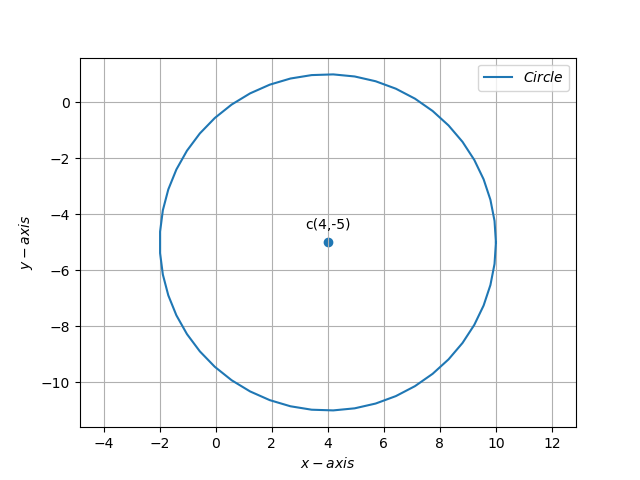
\includegraphics[width=0.75\columnwidth]{chapters/11/11/1/8/figs/11.1.8.png}
	\end{center}
\caption{}
\label{fig:chapters/11/11/1/8/Fig1}
\end{figure}
\fi
